\scanpage{38}
\mspage{\textcircled{19}}
\[
(67)\qquad u(\widetilde d_i^{\prime\omega})=\varphi_i^{\omega'}(\underbrace{\zeta'}_{\eta\zeta})\widetilde d_i^{\prime\omega}
\]
We also have paths
\diagram{\begin{tikzcd}[ampersand replacement=\&,column sep=large,row sep=large]
P^\omega\arrow[rr,"d_i^\omega"]\arrow[dr,"d_{\omega'i}^\omega"']\&\&R_i^\omega\\
\&Q_{\omega'i}\arrow[ur,"c_{\omega'i}^{\omega'}"']\&
\end{tikzcd}}\quad(66')
\[
d_i^\omega=c_{\omega'i}^{\omega'}\cdot d_{\omega'i}^\omega
\]
\margin{\diagram{\begin{tikzcd}[ampersand replacement=\&,column sep=small,row sep=large]
\&P_\infty^\omega\arrow[d,"d_{\omega'i}^\omega"]\arrow[dl,dashed]\\
R_i^\omega\&Q_{\omega'i}\arrow[l,bend left=15,"c_{\omega'i}^{\omega'}"]
\end{tikzcd}}}
\margin{NB $\tau(d_i^\omega)=d_i^{\prime\omega}$}
and we shall also have
\[
(67')\qquad u(\widetilde d_i^\omega)=\varphi_i^\omega(\eta\widetilde\sigma_\infty(\zeta))\widetilde d_i^\omega
\]
\figure{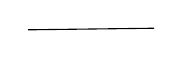
\begin{tikzpicture}\draw (0,0)--(1.6,.02);\end{tikzpicture}}

I see two more cases to look at, namely the full subgroupoids of $\overline{\underline{\mathrm{VI}}}$ induced on the \inserted{eight} vertices $(R_{i,\omega},P^\omega)$, that is $\overline{\underline{\mathrm{VII}}}$, described by the graph of the same name and the arrows $d_i^{\prime\omega},d_i^\omega,a_i^\omega,b_i^\omega$ (24 arrows), and the one induced on the \deleted{five points} \inserted{vertices} $Q_i,P^\omega$ --- strictly speaking, this is the groupoid already named $\overline{\underline{\mathrm{IV}}}$ having the same \deleted{objects} vertices, but
\figure{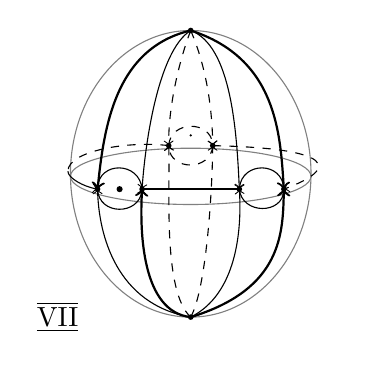
\begin{tikzpicture}[scale=.65]
\draw[gray] (0,0) ellipse (2.35 and 2.8);\draw[gray] (0,-.05) ellipse (2.35 and .55);
\coordinate (P) at (0,2.8);\coordinate (M) at (0,-2.8);
\coordinate (A) at (-1.82,-.3);\coordinate (B) at (-.95,-.3);
\coordinate (C) at (-.43,.55);\coordinate (D) at (.43,.55);
\coordinate (E) at (.95,-.3);\coordinate (F) at (1.82,-.3);
\foreach \p in {P,M,A,B,C,D,E,F}{\fill (\p) circle (.055);}
\draw[thick,->] (P)..controls (-1.5,2.45) and (-1.7,.85)..(A);
\draw[->] (P)..controls (-.65,2.4) and (-.9,.5)..(B);
\draw[dashed,->] (P)..controls (-.25,2.15) and (-.44,1.25)..(C);
\draw[dashed,->] (P)..controls (.3,2.1) and (.42,1.3)..(D);
\draw[->] (P)..controls (.8,2.5) and (.9,.8)..(E);
\draw[thick,->] (P)..controls (1.7,2.25) and (1.75,.75)..(F);
\draw[->] (M)..controls (-1.45,-2.55) and (-1.8,-1.2)..(A);
\draw[thick,->] (M)..controls (-.95,-2.7) and (-1,-1.15)..(B);
\draw[dashed,->] (M)..controls (-.55,-2.3) and (-.4,-.3)..(C);
\draw[dashed,->] (M)..controls (.3,-2.25) and (.42,-.4)..(D);
\draw[->] (M)..controls (.9,-2.35) and (1,-1.1)..(E);
\draw[thick,->] (M)..controls (1.8,-2.25) and (1.8,-1.15)..(F);
\draw[<-] (B)..controls (-1,-.82) and (-1.8,-.82)..(A);
\draw[->] (B)..controls (-1,.25) and (-1.8,.25)..(A);
\draw[dashed,->] (C)..controls (-.4,1.05) and (.4,1.05)..(D);
\draw[dashed,->] (D)..controls (.4,.05) and (-.4,.05)..(C);
\draw[<-] (E)..controls (1,.25) and (1.8,.25)..(F);
\draw[->] (E)..controls (1,-.8) and (1.8,-.8)..(F);
\draw[thick] (B)--(E);
\draw[dashed] (C)..controls (-1.2,.65) and (-2.4,.45)..(-2.4,.05);\draw[->] (-2.4,.05)..controls (-2.4,-.08) and (-2.1,-.25)..(A);
\draw[dashed,->] (D)..controls (2.85,.5) and (2.9,.1)..(F);
\fill (-1.39,-.3) circle (.06);\fill (0,.75) circle (.025);
\node at (-2.6,-2.8) {$\overline{\underline{\mathrm{VII}}}$};
\end{tikzpicture}}
\margin{\uline{NB} the $b_i^\omega$ directly joining the $Q_i$ are unnecessary here}
\figure{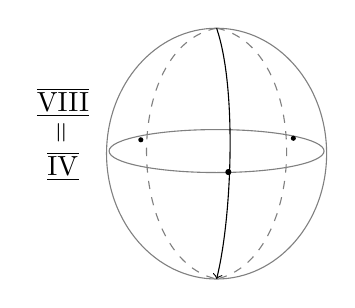
\begin{tikzpicture}[scale=.65]
\draw[gray] (0,0) ellipse (2.15 and 2.45);
\draw[gray] (0,.05) ellipse (2.1 and .42);
\draw[gray,dashed] (0,2.45)..controls (-1.85,2.1) and (-1.8,-2.05)..(0,-2.45);
\draw[gray,dashed] (0,2.45)..controls (1.85,2.1) and (1.8,-2.05)..(0,-2.45);
\draw[->] (0,2.45)..controls (.4,1.3) and (.3,-1.25)..(0,-2.45);
\fill (-1.48,.27) circle (.05);\fill (1.5,.3) circle (.05);\fill (.23,-.36) circle (.06);
\node at (-3,1) {$\overline{\underline{\mathrm{VIII}}}$};\node[rotate=90] at (-3,.4) {$=$};\node at (-3,-.25) {$\overline{\underline{\mathrm{IV}}}$};
\end{tikzpicture}}
represented by a slightly larger graph --- in $\boxed{\mathrm{VIII}}$ one distinguishes the \inserted{six} \deleted{arrows} $d_i^\omega$ only, and one does not in addition give the $\widetilde a_i^\omega$, which is in fact unnecessary by (35). (Thus it is not surprising that in (37), \unsure{the|the} datum of $\widetilde\alpha$, which
\margin{37}
